\begin{figure}
    \centering
\begin{tikzpicture}
    \node [above right, inner sep=0] (image) at (0,0) {
        % Image to annotate
        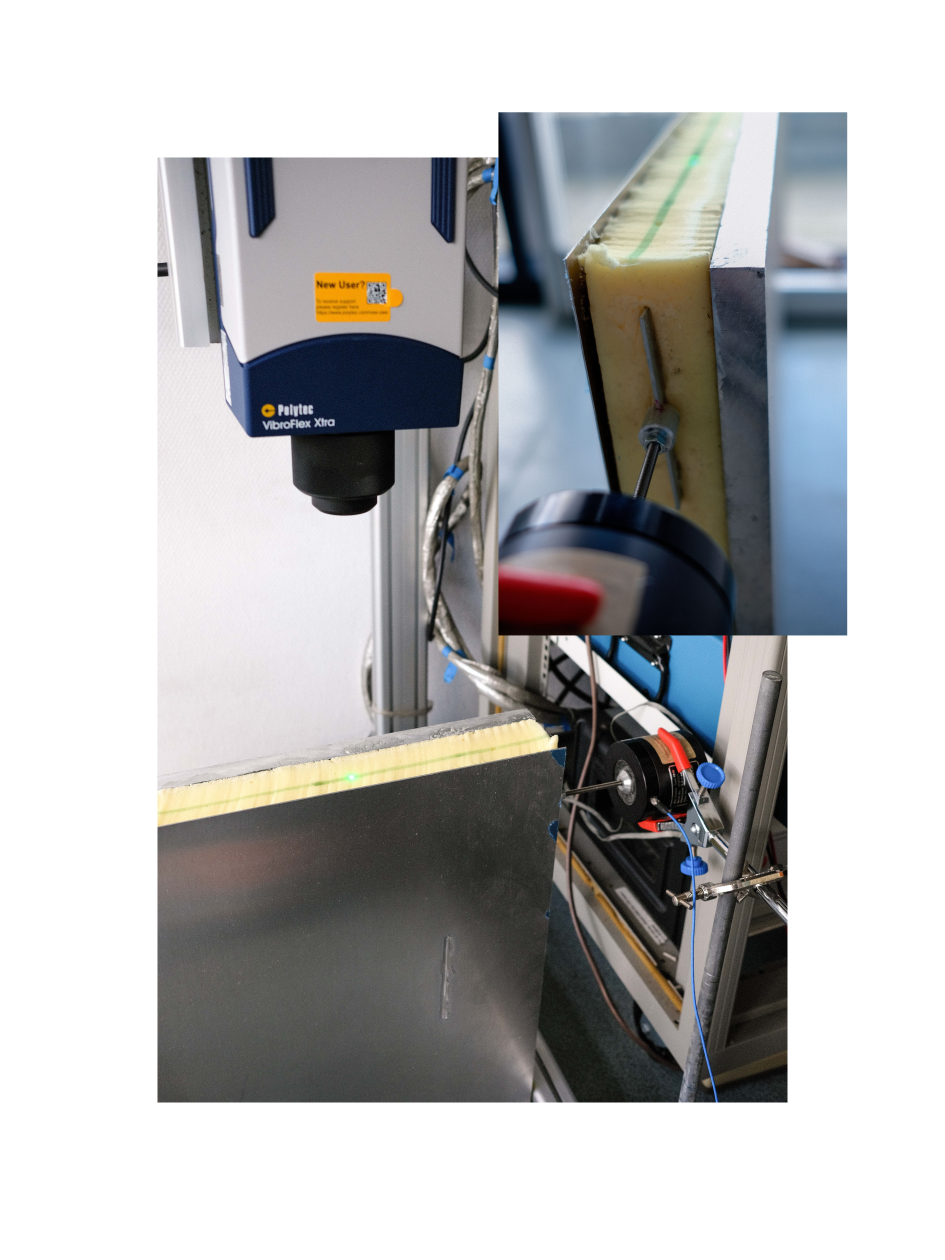
\includegraphics{figures/expe_setup.png}
    };
    % Coordinate scope: 
    %       (0, 0)   bottom left corner of the image 
    %       (10, 10) upper right corner

    \begin{scope}[
        x={($0.1*(image.south east)$)}, 
        y={($0.1*(image.north west)$)}
    ]
        % Put a grid to compute coordinates easily
        % Remove when finished 
        %    \draw[lightgray,step=1] (image.south west) grid (image.north east);
        %    \foreach \x in {0,1,...,10} {
        %        \node [below] at (\x,0) {\x}; 
        %    }
        %    \foreach \y in {0,1,...,10} {
        %        \node [left] at (0,\y) {\y};
        %    }
 
        % Elements  annotation
        \draw[Circle-,very thick,nicecolorfigure] 
            (3, 8) -- ++(0,1.2) node[above, black]{\small Vibrometer};
        \draw[Circle-,very thick,nicecolorfigure] 
            (3.2, 3.9) -- ++(0,-1) node[below, white]{\small Scan line};
        \draw[Circle-,very thick,nicecolorfigure] 
            (7.2, 3.8) -- ++(0,-1.5) node[below, white]{\small Shaker};
        \draw[Circle-,very thick,nicecolorfigure] 
            (6.7,8.5) -- ++(-0.9,1) node[above, black]{\small Plate};
        \draw[Circle-,very thick,nicecolorfigure] 
            (7.4,8.5) -- ++(-0.58, 1.7) node[above, black]{\small Foam};
        \draw[Circle-,very thick,nicecolorfigure] 
            (7.9,8.5) -- ++(0.4,1) node[above, black]{\small Backing} ;
        % Shapes 
        \draw[very thick,nicecolorfigure] (5, 3.2) rectangle (7, 4.5); 
        \draw[very thick,nicecolorfigure] (5, 4.5) -- (5.3,4.95); 
        \draw[very thick,nicecolorfigure] (7,4.5) -- (8.95,4.95);
        \draw[very thick,nicecolorfigure] (5.3,4.95) rectangle (8.95,9.1);
    \end{scope}
    \node[above right] at (6, 0.85) {\includegraphics[scale=.96]{figures/fig_expe.pdf}};
    \node[above left] at (1.5, 8) {a)};
    \node[above left] at (7.5, 8) {b)};
    \node[above left] at (12.3, 8) {c)};
\end{tikzpicture}
\caption{a) Experimental set-up used for the measurement of the normal displacement field of the two-layer structure, with a close-up of the sample excitation. b) Real and c) imaginary parts of the dispersion relations recovered experimentally from the SLaTCoW method (black crosses) as calculated with the SCM (colored lines) and the bulk wavenumbers in the poroelastic material (magenta lines).}
\label{fig:expe}
\end{figure}